%%%%%%%%%%%%%%%%%%%%%%%%%%%%%%%%%%%%%%%%%%%%%%%%%%%%%%%
%%% 美国大学生数学建模竞赛(MCM/ICM)论文模板
%%% 来源网站:www.latexstudio.net
%%% 中文注释:小嗷犬 blog.marquis.eu.org
%%%%%%%%%%%%%%%%%%%%%%%%%%%%%%%%%%%%%%%%%%%%%%%%%%%%%%%
%%% code: 代码文件夹
%%% figures: 图片文件夹
%%% *.cls: LaTeX 格式文件
%%% *.tex: LaTeX 文档文件
%%% *.bib: Bib 引用文献源文件
%%%%%%%%%%%%%%%%%%%%%%%%%%%%%%%%%%%%%%%%%%%%%%%%%%%%%%%

%%%%%%%%%%%%%%%%%%%%%%%%%%%%%%%%%%%%%%%%%%%%%%%%%%%%%%%
%%% 可能用到的网站
%%%%%%%%%%%%%%%%%%%%%%%%%%%%%%%%%%%%%%%%%%%%%%%%%%%%%%%
%%% LaTeX公式编辑器:https://www.latexlive.com/
%%% Diagram流程图绘制:https://www.drawio.com/
%%%%%%%%%%%%%%%%%%%%%%%%%%%%%%%%%%%%%%%%%%%%%%%%%%%%%%%

%%%%%%%%%%%%%%%%%%%%%%%%%%%%%%%%%%%%%%%%%%%%%%%%%%%%%%%
%%% 模板参数设置
%%%%%%%%%%%%%%%%%%%%%%%%%%%%%%%%%%%%%%%%%%%%%%%%%%%%%%%
\documentclass{mcmthesis}  % 文档类型
\usepackage{float} % 引入float宏包,提供H选项功能
\mcmsetup{CTeX = false,   % 使用 CTeX 套装时,设置为 true
        tcn = 2501262,   % 队伍控制号
        problem = C,  % 选题
        sheet = true,   % sheet页
        titleinsheet = true,   % sheet页显示标题
        keywordsinsheet = true,  % sheet页显示关键词
        titlepage = false,   % 标题页
        abstract = true  % 摘要
        }
%%%%%%%%%%%%%%%%%%%%%%%%%%%%%%%%%%%%%%%%%%%%%%%%%%%%%%%

%%%%%%%%%%%%%%%%%%%%%%%%%%%%%%%%%%%%%%%%%%%%%%%%%%%%%%%
%%% 导入宏包和引用文献源
%%%%%%%%%%%%%%%%%%%%%%%%%%%%%%%%%%%%%%%%%%%%%%%%%%%%%%%
\usepackage{palatino}  % 帕拉提诺体字体宏包
\usepackage{lipsum}  % 导入生成段落的宏包
\usepackage[hyperref=true,style=ieee]{biblatex}  % biblatex参考文献宏包
\addbibresource{ref.bib}  % 添加引用文献bib源
%%%%%%%%%%%%%%%%%%%%%%%%%%%%%%%%%%%%%%%%%%%%%%%%%%%%%%%

%%%%%%%%%%%%%%%%%%%%%%%%%%%%%%%%%%%%%%%%%%%%%%%%%%%%%%%
%%% 文档信息设置
%%%%%%%%%%%%%%%%%%%%%%%%%%%%%%%%%%%%%%%%%%%%%%%%%%%%%%%
\title{Prediction of Olympic Medal Ranks Based on Random Forest and FEM Model}  % 文章标题
\author{\small Team 2501262}  % 作者,开启标题页才会显示
\date{\today}  % 日期,开启标题页才会显示

\memoto{MCM office}  % 建议书目标
\memofrom{MCM Team 2501262}  % 建议书来源
\memosubject{MCM}  % 建议书主题
\memodate{\today}  % 建议书日期
%%%%%%%%%%%%%%%%%%%%%%%%%%%%%%%%%%%%%%%%%%%%%%%%%%%%%%%

%%%%%%%%%%%%%%%%%%%%%%%%%%%%%%%%%%%%%%%%%%%%%%%%%%%%%%%
%%% 文档开始
%%%%%%%%%%%%%%%%%%%%%%%%%%%%%%%%%%%%%%%%%%%%%%%%%%%%%%%
\usepackage{subcaption}
\usepackage{setspace}
\usepackage{etoolbox}
\usepackage{float}
\renewcommand{\contentsname}{Contents}

\AtBeginDocument{
    \let\oldtableofcontents=\tableofcontents
    \renewcommand{\tableofcontents}{
        \begingroup
        \setstretch{0.5} % 仅目录行间距设为0.9倍
        \oldtableofcontents
        \endgroup
    }
}


\begin{document}  % 文档
\begin{abstract}  % 摘要
\hspace*{1.5em}In 2024, the spectacular opening ceremony of the French Olympics captivated the attention of millions worldwide. At this quadrennial extravaganza, the ultimate victors stood atop the podium, basking in the cheers and applause of countless admirers. This spectacle naturally sparked widespread curiosity: how can we predict who will claim the medals and revel in this supreme honor? Thus, our team has developed mathematical models aimed at analyzing and forecasting the medal standings for the 2028 Olympics, offering strategic  recommendations for nations to cultivate future champions.

\textbf{In Model 1}, for countries with \textbf{more than one medal}, we first calculated their project scores using the entropy weight method and the TOPSIS method. These scores were then used to train a random forest model to predict the number of medals each country might achieve. For countries with\textbf{ no more than one medal}, we employed logistic regression to estimate the probability of winning their first medal. The results indicate that most countries, such as the United States and China, are likely to \textbf{improve their performance}, while a few, like Guatemala, may experience a decline. Additionally, our model suggests that \textbf{11 countries} could potentially win their first-ever medals.

\textbf{In Model 2}, when studying the relationship between the host country and the number of medals won, we constructed a fixed effect regression model estimated the parameters using OLS method. The results show that the host country has a significant advantage in the Olympic Games, and the advantage is more obvious in the new events.

\textbf{In Model 3}, we employed an event study regression model combined with a t-test to compare the differences in national medal counts between scenarios with and without renowned coaches, thereby quantifying the impact of coach introductions on Olympic medal outcomes. The results revealed that events such as gymnastics and volleyball experienced \textbf{a significant increase} in medal counts following the introduction of outstanding coaches, with the intervention effects demonstrating both dynamism and persistence. Furthermore, our study predicts that the introduction of exceptional coaches will have a substantial positive impact on medal count growth in events such as Brazilian athletics, Indian badminton singles, and Vietnamese women's weightlifting.

The sensitivity analysis results show that the model exhibits significant robustness across varying noise levels and maintains commendable performance. These findings provide critical insights for nations to formulate strategic sports development policies and enhance their competitive edge in the Olympic Games and the broader sports arena.
\begin{keywords}  % 关键词
Olympic Games medal prediction; TOPSIS; Random Forest; Logistic; FEM
\end{keywords}  % 结束关键词
\end{abstract}  % 结束摘要
\maketitle  % 生成sheet页

\tableofcontents  % 生成目录表

%%%%%%%%%%%%%%%%%% sheet页与目录页结束 %%%%%%%%%%%%%%%%%%

\newpage  % 开始新的一页
\section{Introduction}  % 一级标题

\subsection{Background}  % 二级标题

\hspace*{1.5em}Currently, Olympic medal predictions tend to focus on information about athletes and teams closer to the games. However, historical performance data, such as the number of MEDALS won in the past, different sports settings, etc., may provide greater insight into medal predictions. Therefore, it is crucial to build a model that can assess trends in the number of MEDALS, identify countries that are likely to win MEDALS for the first time, and explore the impact of specific sports, sports, and even coaching on competition results. These insights could inform the strategic decisions of national Olympic committees for future Games.
\begin{figure}[h]  % 图片
\small
\centering  % 居中
\includegraphics[width=10cm]{B.png}  % 引入图片源
\caption{Olympic Games venue}  % 标题
\end{figure}  % 图片结束

\subsection{Restatement of the Problem}  % 二级标题
\hspace*{1.5em}Considering the background information and the restricted conditions identified in the problem statement, we need to solve the following problems:
\begin{itemize}  % 无序列表
\item Project the medal standings for the Los Angeles Olympics 2028, with prediction intervals for each result, and identify which countries are likely to improve or decline compared to their 2024 performance. Estimate how many countries that have never won a medal might earn their first in 2028, along with the odds of this happening.
\item Analyze the relationship between the number and types of Olympic events and medal counts, identifying key sports for different countries, and how the selection of sports by the host country may influence the results.
\item Explore the potential "great coach" effect, where the success of renowned coaches (e.g., Lang Ping or Béla Károlyi) may impact a country's medal count. We will examine the data for evidence of this effect, estimate its contribution, and suggest which countries might benefit from investing in high-caliber coaches for specific sports.
\end{itemize}  % 无序列表结束

\subsection{Our Work}  % 二级标题

\begin{itemize}  % 无序列表
\item For the countries with more than one medal, we use the entropy weight method TOPSIS and random forest to predict the number of medals and simultaneously determine the importance of the events; For countries with the number of medals being less than or equal to 1, logistic regression is utilized to predict the probability of winning medals.
\item We constructed a fixed-effect regression model, controlling for the fixed effects of countries and years, and estimated the parameters using ordinary least squares. We analyzed the advantages of the host country in terms of new projects.
\item When analyzing the effect of famous coaches, we establish a t-test model to compare the differences in medal counts between the cases with and without famous coaches; we apply the event study regression model to evaluate the dynamic persistence of the effect of famous coaches; and we explore the heterogeneity and internal mechanism of the effect of famous coaches through group regression and the mediation effect model.
\end{itemize}  % 无序列表结束
\begin{figure}[H]  % 图片
\small
\centering  % 居中
\includegraphics[width=12.5cm]{our work.png}  % 引入图片源
\caption{our work} 
\end{figure}  % 图片结束

\section{Assumptions and Justifications}  % 一级标题
\begin{itemize}  % 无序列表
\item Assumption: Assuming that the athletes' performance does not change with age, and ignoring the influence of injuries, training status, etc. on the performance of the athletes.

Justification: The focus of the model is on the prediction of the number of medals won by the country. Temporarily ignoring the influence of age and other factors can highlight the role of core factors such as coaches and event types, avoiding making the model overly complex due to excessive consideration of age factors, and thereby masking the role of core variables.
\item Assumption: Count the gold medals of the team event as individual gold medals for each athlete.

Justification: This model will consistently apply this assumption across all countries, thus enabling a unified comparison of each country's performance and still allowing for tracking of their overall situation based on the total number of medals they have won.
\item Assumption: As the participating athletes for the 2028 Olympic Games have not been announced by various countries yet, we have selected the athletes who participated in the 2020 or 2024 Olympic Games and are under 40 years old as the participants for the 2028 Olympic Games. (This is just to determine the participating athletes based on their ages to explain the results of our model, and it is not used in the model as an influencing factor.)

Justification: Due to the inability to obtain the information of athletes participating in the 2028 Olympic Games at present, it is a more feasible solution to select the relevant data of the athletes for the 2020 or 2024 Olympic Games. We already know the detailed information such as the competition events and results of these athletes, and these data can provide the necessary foundation for establishing a mathematical model.
\item Assumption: Suppose that within the same project type (either individual or team project), the responses of each project to the coaching effect are homogeneous.

Justification: The same type of project usually has similar competitive laws, training patterns, and competition rules. From the overall trend, their responses to the coaching effect are homogeneous. This facilitates grasping the general characteristics of team projects and the commonalities of the coaching effect.
\end{itemize}  % 无序列表结束

\section{Data Processing}  % 一级标题

\subsection{Data Extraction}  % 二级标题
\begin{itemize}  % 无序列表
\item Due to the fact that in `summerOly athletes.csv`, the `Team` section may have different team names for the same country, and our model analysis focuses mainly on the country and event themes, we directly adopt the NOC code of the country instead of dividing by "Team". The NOC code is sufficient to represent the information at the national level and can meet the basic requirements for modeling and analyzing the medal tables of various countries. This ensures the consistency of country identification in the data.
\item We extracted the `discipline` column from `summerOly programs.csv` and used it as the data set for sports events. We renamed it as `Sport` and will not elaborate further.
\item We utilized the Wikidata API.\textsuperscript{\cite{[1]}}  % 引用文献
query the birth years of the contestants in 2020 and 2024 in order to calculate their age.
\end{itemize}  % 无序列表结束
\begin{figure}[H]  % 图片
\small
\centering  % 居中
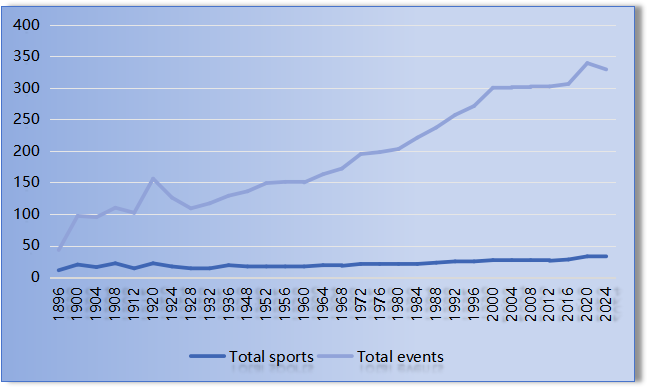
\includegraphics[width=12cm]{a.png}  % 引入图片源
\caption{The variation of project quantity over the years}  % 标题
\end{figure}  % 图片结束


\subsection{Data Cleaning}  % 二级标题
\begin{itemize}  % 无序列表
\item Check for missing values in each dataset. If the proportion of missing values is small, delete the corresponding records; if it is large, fill in the missing values. For duplicate data, if they are consistent, delete the duplicate records; if they are inconsistent, verify the data sources and select the accurate ones.
\item "Mixed Team" refers to a team composed of athletes from different countries. Since it is impossible to predict the medal-winning performance of each country based on this team, it is excluded from consideration.
\item Netherlands Antilles has now disintegrated and no longer appears as an independent competitor in events such as the Olympics, so it is omitted.
\end{itemize}  % 无序列表结束

\subsection{Merge the Data Sets}  % 二级标题
\begin{itemize}  % 无序列表
\item Sort out a new table based on the country's NOC as the first key word, the sport as the second key word, and the athlete's name as the third key word in lexicographical order. This will result in a table showing the total number of medals and the number of gold, silver and bronze medals each athlete has obtained throughout their career, the number of medals each country has won in each event each year, and the total number of medals each country has won each year.
\item Merge the data of athletes, hosts and events, filter out the records without awards, and mark the newly added events (the years when they first appeared) and the host countries. Aggregate the number of medals by country-year-event and control the total number of medals in history to exclude the "zero-medal countries".
\item We have consolidated the competition records of some countries, such as merging East Germany and West Germany into Germany. This approach enables a more comprehensive consideration of the situation of sport development in each country, avoiding loss of information or bias caused by division. At the same time, it improves the accuracy and reliability of the model, providing stronger support to predict and analyze the performance of this country in future sporting events.
\end{itemize}  % 无序列表结束
\subsection{Feature Engineering}  % 二级标题
\begin{itemize}  % 无序列表
\item Based on the performance of each country in past Olympic Games, we classified the data into two categories: those with more than one medal and those with less than one. This is to prepare for the establishment of the model.
\end{itemize}  % 无序列表结束
%%%%%%%%%%%%%%%%%%%%%%%% 并排图 %%%%%%%%%%%%%%%%%%%%%%%%
\begin{figure}[H]
\centering
\subcaptionbox{Total Medal Count\label{fig:total}}{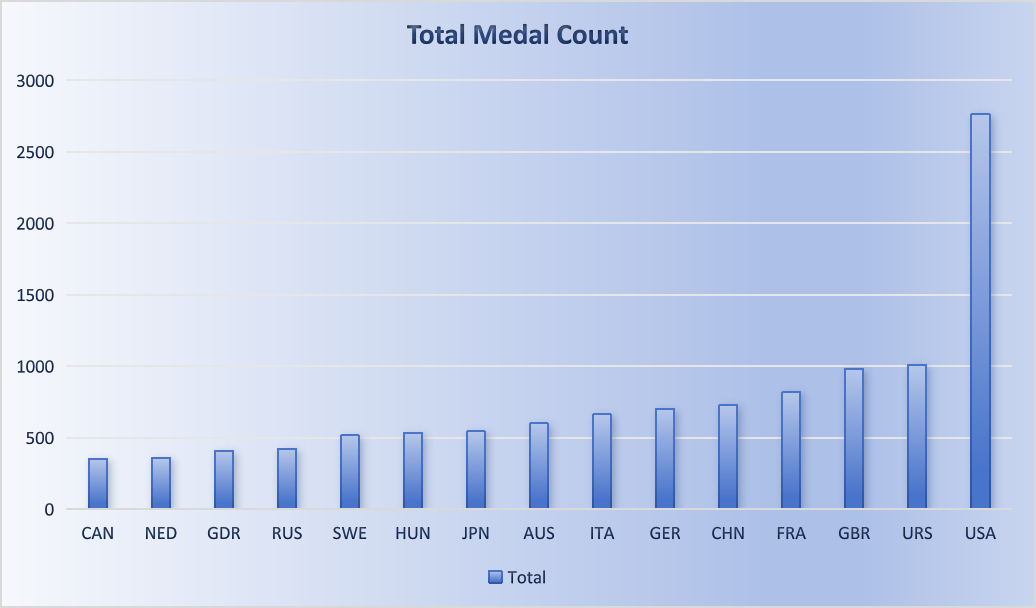
\includegraphics[width=0.48\textwidth]{total.png}}
\hfill
\subcaptionbox{Medal Count by Region\label{fig:region}}{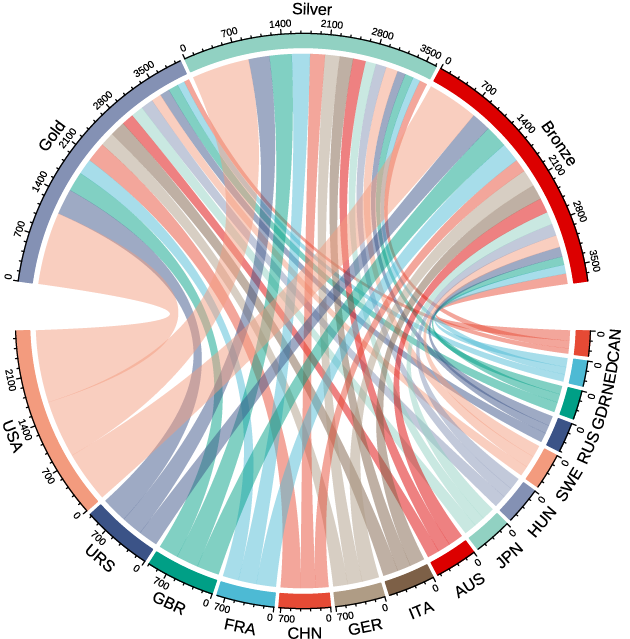
\includegraphics[width=0.48\textwidth]{jp.png}}
\caption{The Situation of Medal Awards}
\label{fig:sidebyside}
\end{figure}
%%%%%%%%%%%%%%%%%%%%%% 并排图结束 %%%%%%%%%%%%%%%%%%%%%%
\section{Model 1: Prediction of the 2028 Olympic Medal Table}  % 一级标题模型1

\subsection{Model Establishment}  % 二级标题
\subsubsection{Countries with More than One Medals}  %三级标题
\hspace*{1.5em}By applying the entropy weight method and TOPSIS method, based on the number of each type of medal (gold, silver and bronze) for each country for each event, the conversion rate of each type of medal (that is, the ratio of the number of medals won by a country to the number of participants of that country), and the participation rate of each event for each country, the score of each event is calculated, and the importance of each event to the country is determined by the ranking of the scores. Let the number of evaluation objects be \(m\), the number of evaluation indicators be \(n\), and the original data matrix be \(X = (x_{ij})_{m \times n}\). To eliminate the influence of scale, the data are standardized. The formula is $$z_{ij} = \frac{x_{ij} - \min_{i}(x_{ij})}{\max_{i}(x_{ij}) - \min_{i}(x_{ij})}$$. Calculate the information entropy \(e_j\) of the \(j\)-th indicator, the formula is $$e_j = -k \sum_{i = 1}^{m} p_{ij} \ln(p_{ij}), (k = \frac{1}{\ln(m)}, p_{ij} = \frac{z_{ij}}{\sum_{i = 1}^{m} z_{ij}}) $$If \(p_{ij} = 0\), it is stipulated that \(p_{ij} \ln(p_{ij}) = 0\). Calculating the entropy weight \(w_j\) of the \(j\)-th indicator, the formula is $w_j = \frac{1 - e_j}{\sum_{j = 1}^{n} (1 - e_j)}$, satisfying \(\sum_{j = 1}^{n} w_j = 1\). Determine the positive ideal solution \(Z^+\) and the negative ideal solution \(Z^-\): \[Z^+ = (\max_{i}z_{i1},\max_{i}z_{i2},\cdots,\max_{i}z_{in}), Z^- = (\min_{i}z_{i1},\min_{i}z_{i2},\cdots,\min_{i}z_{in})\]
Calculate the distances \(D_i^+\) and \(D_i^-\) of each evaluation object from the positive and negative ideal solutions. \[D_i^+=\sqrt{\sum_{j = 1}^{n}w_j(z_{ij}-z_{j}^+)^2},D_i^-=\sqrt{\sum_{j = 1}^{n}w_j(z_{ij}-z_{j}^-)^2}\]
Finally, calculate the comprehensive evaluation score \(C_i\): $C_i=\frac{D_i^-}{D_i^++D_i^-}$
The larger the value of \(C_i\), the better the evaluated object.

By using the same method, we will combine the medal-winning records of all the participating athletes in 2020 and 2024 into the same table (if an athlete participated in both the 2020 and 2024 Olympics, we will list the data up to 2020 and the data up to 2024 separately for each of them in the table), and calculate the comprehensive score of each athlete based on the total number of medals and the total number of competitions.
Then, based on the competition projects in 2028 and the strength ranking of the participating team members, we select the corresponding number of participants for each country to compete in the event. Thus, we can conveniently calculate the total score of athletes who participate in each event for each country.

After obtaining the above information, we use the TOPSIS total scores of each project for each country up to 2020, the number of medals of all participating contestants in each event and the proportion of medals to the total number of medals in each event in 2020, whether the country is the host country, and the above information up to 2016 as independent variables, and the number of medals obtained by the country in each event in 2024 and 2020 as dependent variables to train the random forest model.

\subsubsection{Countries with no more than One Medals}  %三级标题
\hspace*{1.5em}For countries that have not yet won a gold medal, a logistic regression is performed using the number of competitions and the number of events participated in before obtaining the first medal to calculate the probability of winning a gold medal.

\subsection{Model Training}  % 二级标题
\hspace*{1.5em}When training of the random forest model is performed first, the data set is divided into a training set (80\%) and a test set (20\%) in an 8: 2 ratio. Then, grid search and cross-validation are used to optimize the hyperparameters. Finally, the following configurations are selected, as shown in Table 1:
%%%%%%%%%%%%%%%%%%%%%%%% 三线表 %%%%%%%%%%%%%%%%%%%%%%%%
\begin{table}[H]  % 表格
\caption{configurations}  % 标题
\label{tab1}  % 标签
\tabcolsep 15pt % 列间距s
\begin{tabular*}{\textwidth}{cc}  % tabular*环境
\toprule  % 顶线
Number of decision trees (n estimators): & 200 \\
\midrule  % 中线
Maximum depth (max depth): & 10 \\
\midrule  % 中线
Minimum number of samples for leaf nodes (min samples leaf):&5\\
\midrule  % 中线
 Minimum number of samples for split (min samples split):&10\\
\bottomrule  % 底线
\end{tabular*}  % tabular*环境结束
\end{table}  % 表格结束
%%%%%%%%%%%%%%%%%%%%%% 三线表结束 %%%%%%%%%%%%%%%%%%%%%%

We train the random forest model based on Python using the training set, and the code is shown in appendix A. The results obtained are: $R^2$ Score = $0.692$ and MAE = $0.198$. This indicates that the model has a relatively good prediction result.

\subsection{The Predicted Results of Data Related to the 2028 Olympic Games}  % 二级标题
\begin{itemize}  % 无序列表
\item Prediction of the Medal Table:

Based on the total number of medals and the quantities of each type of medals, we predict that the performances of different countries will vary, and the degree of progress for each country that has made progress will also be different. Most countries are making progress, such as the United States, the United Kingdom, France, Canada and China. However, some countries are regressing, such as Guatemala and Dominica. Overall, the sports powerhouses are all making progress, which may be related to their abundant experience, rich sports resources and numerous outstanding talents, as shown in Figure 5. 
\begin{figure}[H]  % 图片
\small
\centering  % 居中
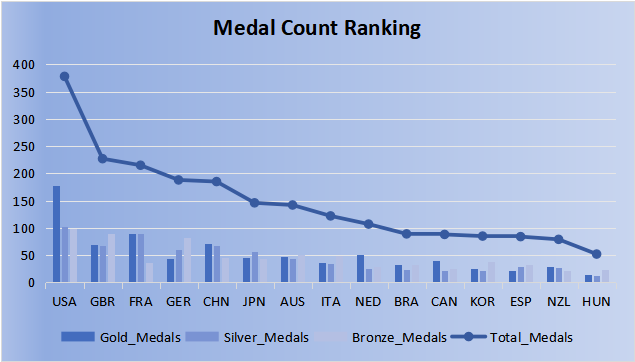
\includegraphics[width=14cm]{2028.png}  % 引入图片源
\caption{Medal Count Ranking}  % 标题
\end{figure}  % 图片结束

\item Prediction of the First Medal-Winning Country:

It is predicted that 11 countries will win the first medal at the next Olympic Games. They are Angola (ANG), Bolivia (BOL), El Salvador (ESA), Honduras (HON), Liechtenstein (LIE), Madagascar (MAD), Mali (MLI), Malta (MLT), Myanmar (MYA), Nicaragua (NCA) and Sierra Leone (SLE). The Figure 6 shows the probabilities of the correct predictions.
\begin{figure}[H]  % 图片
\small
\centering  % 居中
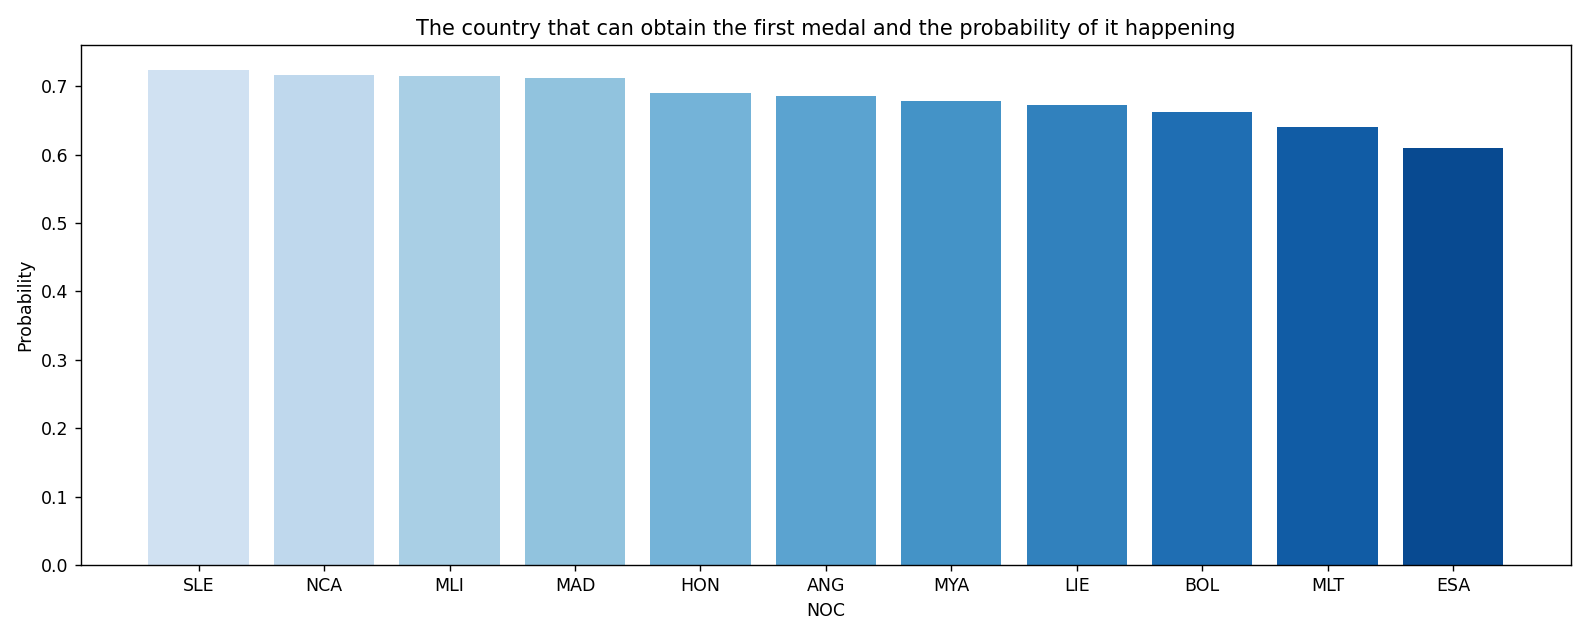
\includegraphics[width=14cm]{probability.png}  % 引入图片源
\caption{The country that can obtain the first medal and the probability of it happening}  % 标题
\end{figure}  % 图片结束

\item The Influence of the Chosen Projects on  the Number of medals:

The degree of attention paid by different countries to various sports events varies, reflecting the characteristics and priorities of each country in sports development. Sports powerhouses usually attach importance to the development of multiple sports to comprehensively enhance the country's sports strength and international competitiveness; while some small countries may focus on developing a few sports based on their own resources and advantages. For example, track and field are highly valued and score relatively high in sports powerhouses such as the United States. Although Liechtenstein is a small country, it has a mountainous terrain and thus achieved good results in the Cycling Mountain Bike event. To some extent, the choice of important sports by each country will increase their chances of winning more medals.As shown in Table 2 and Figure 7.

%%%%%%%%%%%%%%%%%%%%%%%% 三线表 %%%%%%%%%%%%%%%%%%%%%%%%
\begin{table}[H]  % 表格
\caption{The Significance of Different Projects to Different Countries}  % 标题
\tabcolsep 30pt % 列间距
\begin{tabular*}{\textwidth}{cccc}  % tabular*环境
\toprule  % 顶线
NOC & Sport & Score & Rank \\
\midrule  % 中线
USA & Athletics & 0.731769839 & 1 \\
\midrule  % 中线
LIE & Cycling Mountain Bike & 0.541932005 & 1 \\
\midrule  % 中线
BER & Boxing & 0.532894185 & 1 \\
\midrule  % 中线
BRA & Football & 0.713704545 & 1 \\
\midrule  % 中线
CHI & Tennis & 0.496399218 & 1 \\
\midrule  % 中线
\multicolumn{4}{c}{Note: Due to the abundance of data, only representative data are listed here.}
\end{tabular*}  % tabular*环境结束
\end{table}  % 表格结束
%%%%%%%%%%%%%%%%%%%%%% 三线表结束 %%%%%%%%%%%%%%%%%%%%%%
\begin{figure}[H]  % 图片
\small
\centering  % 居中
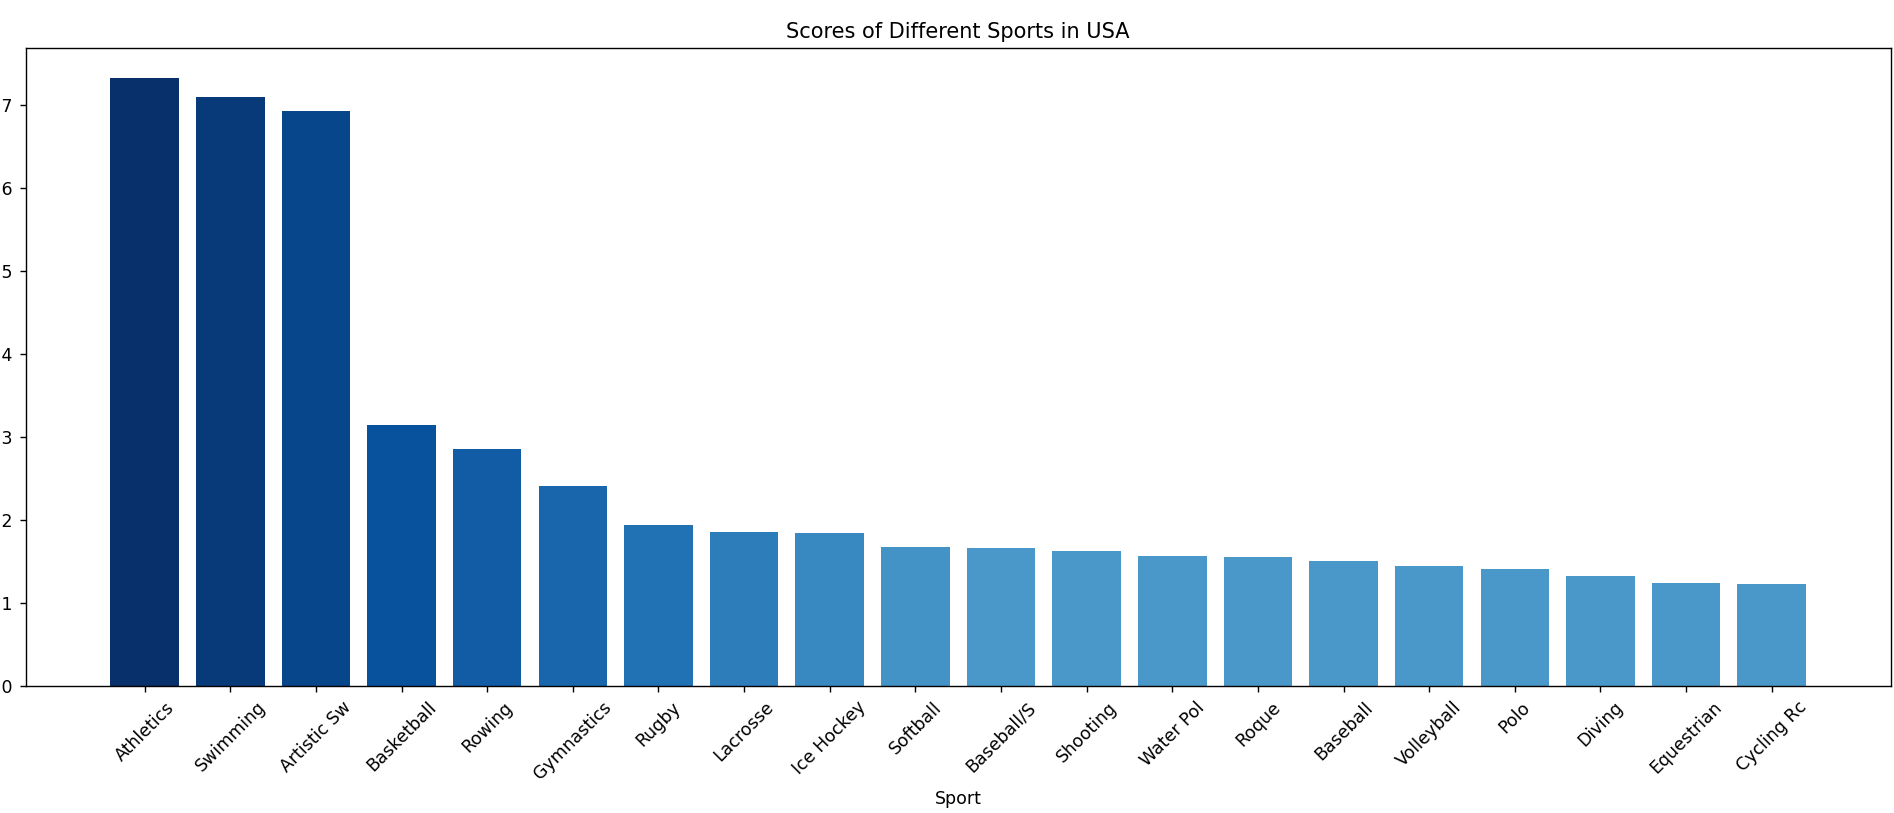
\includegraphics[width=14cm]{usa.png}  % 引入图片源
\caption{The significance of different projects to the United States}  % 标题
\end{figure}  % 图片结束

\end{itemize}  % 无序列表结束

\section{Model 2: The Relationship between the Host Country and the Number of Medals Won}  % 一级标题模型1.5
\subsection{Model Establishment}  %二级标题
\hspace*{1.5em}The variables involved in our solution process are Host( Binary variable, 1 if a country is the host of the Olympic Games in a specific year, 0 otherwise), NewEvent( Binary variable, 1 if a sport is introduced as a new event in that year, 0 otherwise), Total( Total medals (gold, silver, bronze) won by a country in a specific sport and year), Country Fixed Effects( Controls for inherent differences in sports traditions and resource investments across countries), Year Fixed Effects( Controls for temporal factors such as the scale of the Olympics and participant numbers). We construct the following fixed effect regression model: \[
\text{Total} = \beta_0 + \beta_1 \text{Host} + \beta_2 \text{NewEvent} + \beta_3 (\text{Host} \times \text{NewEvent}) + \text{C(NOC)} + \text{C(Year)} + \epsilon\]
\hspace*{1.5em}Use interaction terms( Host × NewEvent) to test whether the host country has additional advantages in the new projects; eliminate unobserved heterogeneity through country and year fixed effects, that is, control variables.Then, the ordinary least squares (OLS) method is employed to estimate the model parameters. The dependent variable is the total number of medals (here, referring to the total number of medals won by a certain country in a single event in a specific year), and the independent variables include host, NewEvent, and their interaction terms. The fixed effects of countries and years are achieved through dummy variables to eliminate cross-temporal systematic biases.

\subsection{Result}  %二级标题
\hspace*{1.5em}The Relationship Between the Host Country and the Number of Medals Won:
%%%%%%%%%%%%%%%%%%%%%% 表开始 %%%%%%%%%%%%%%%%%%%%%%
\begin{table}[H]
\centering
\caption{OLS Regression Results}
\begin{tabular}{|c c|c c|}
\hline
Indicators & Numerical value & Indicators & Numerical value \\
\hline
Dep. Variable: & Total & R - squared: & 0.742 \\
\hline
 Model: & OLS & Adj. R - squared: & 0.741 \\
\hline
 Method: & Least Squares & F - statistic: & 1528 \\
\hline
 Date: & Sun, 26 Jan 2025 & Prob (F - statistic): & 0.00 \\
\hline
Time: & 15:30:29 & Log - Likelihood: & - $4.5844\times 10^{5}$ \\
\hline
 No. Observations: & 99240 & AIC: & $9.173\times 10^{5}$ \\
\hline
 Df Residuals: & 99053 & BIC: & $9.190\times 10^{5}$ \\
\hline
Df Model: & 186 & Covariance Type: & nonrobust  \\
\hline
\end{tabular}
\end{table}
%%%%%%%%%%%%%%%%%%%%%% 表结束 %%%%%%%%%%%%%%%%%%%%%%
We obtained the results. The Beta coefficient of Host is 88.3957 and the P value is 0.000. The coefficient is significant, indicating that the host country has a significant advantage. The B coefficient of Host × NewEvent is 13.3605 and the P value is 0.000. The coefficient is also significant. The host country also has a significant advantage in new projects. This suggests that the host country may have a strategic advantage in new projects due to its early investment in training resources and improve medal performance.


\section{Model 3: Exploring the Effect of Famous Coaches}  % 一级标题模型2
\subsection{The influence of the effect of famous coaches on the number of medals won}  % 二级标题
\subsubsection{T-test Model}

\hspace*{1.5em}To investigate whether the medal count of the treatment group (with 'Great Coach') is significantly higher than that of the control group (without 'Great Coach'), we established a t-test model to test the difference in the average medal count between the treatment group and the control group. The null hypothesis ($H_0$) is that there is no difference in the average medal count between the treatment group and the control group (\(\mu_{\text{Treated}} = \mu_{\text{Control}}\)); the alternative hypothesis ($H_1$) is that the average medal count of the treatment group is higher than that of the control group (\(\mu_{\text{Treated}} > \mu_{\text{Control}}\)). We selected the following coaches:
\begin{itemize}  % 无序列表
\item Sandro Damilano: Italian track and field coach, who became the coach of the Chinese track and field team in 2008 and won a gold medal and a bronze medal at the 2012 Olympics, and a gold medal and a silver medal at the 2016 Olympics.
\item Wang Tongxiang: Chinese diving coach who later became the coach of the Australian diving team, helping the Australian diving team win a gold medal at the 2004 Olympics.
\item Lang Ping: She coached the US women's volleyball team in 2005 and returned to China to coach again in 2013, leading the US team and the Chinese team to win the volleyball championship, respectively.
\end{itemize}  % 无序列表结束
\hspace*{1.5em}Extract the medal counts of all combinations of countries, events, and years in the treatment group as the medal count of the treatment group, denoted as the list \(X = [x_1, x_2, \cdots, x_n]\); extract the medal counts of the same event in other countries at the same time as the medal count of the comtrol group, denoted as the list \(Y = [y_1, y_2, \cdots, y_m]\). By calculating the sample means \(\bar{X}\) and \(\bar{Y}\), and the sample variances \(s_X^2\) and \(s_Y^2\), we constructed the t-statistic: \[t = \frac{\bar{X} - \bar{Y}}{\sqrt{\frac{s_X^2}{n} + \frac{s_Y^2}{m}}}\]
And the degrees of freedom are determined approximately by using the Welch - Satterthwaite approximation: \[ \text{df} = \frac{\left( \frac{s_X^2}{n} + \frac{s_Y^2}{m} \right)^2}{\frac{(s_X^2/n)^2}{n-1} + \frac{(s_Y^2/m)^2}{m-1}}
\]
\hspace*{1.5em}Then, based on the t-statistic and degrees of freedom, look up the t-distribution table and use statistical software to calculate the one-sided p-value. Based on this, judge the significance of the difference in the average number of medals between the two groups.

\subsubsection{Significance Test of the Regression Coefficients of the Event Study Method}

\hspace*{1.5em}The regression model is set as follows: $$\text{Treated\_Medals}_{it} = \beta_0 + \beta_{-2} \text{Post}_{-2,it} + \beta_{-1} \text{Post}_{-1,it} + \beta_0 \text{Post}_{0,it} + $$$$\beta_1 \text{Post}_{1,it}+ \beta_2 \text{Post}_{2,it} + \beta_6 \text{Control\_Medals}_{it} + \gamma \cdot \text{Case}_i + \epsilon_{it}$$
Among them, \(\text{Treated\_Medals}_{it}\) represents the number of medals received by the treatment group in country \(i\) and period \(t\); \(\text{Post}_{j,it}\) (where \(j = -2, -1, 0, 1, 2\)) are time dummy variables used to capture the effect of the intervention in different periods; \(\text{Control\_Medals}_{it}\) represents the number of medals received by the control group; \(\text{Case}_i\) is a control variable; \(\epsilon_{it}\) is the term of random error. Using the OLS method, the coefficients of each dummy variable in time (\(\beta_{-2}, \beta_{-1}, \beta_0, \beta_1, \beta_2\)) are estimated. The significance of the coefficients is tested by calculating the standard error (\(SE(\beta_k) = \sqrt{\text{Var}(\beta_k)}\)), confidence interval (\(\beta_k \pm 1.96 \cdot SE(\beta_k)\)), t-statistic (\(t_k = \frac{\beta_k}{SE(\beta_k)}\)), and p-value. At the same time, a joint significance F test is performed to analyze the dynamic persistence of the intervention effect.
$$\beta_{-2} = \beta_{-1} = \beta_0 = \beta_1 = \beta_2 = 0$$
$$F = \frac{(R^2_{\text{full}} - R^2_{\text{restricted}})/q}{(1 - R^2_{\text{full}})/(n - k - 1)}$$
Where \(q = 5\) (the number of constraint variables), \(k\) is the number of variables in the full model.

\begin{figure}[h]  % 图片
\small
\centering  % 居中
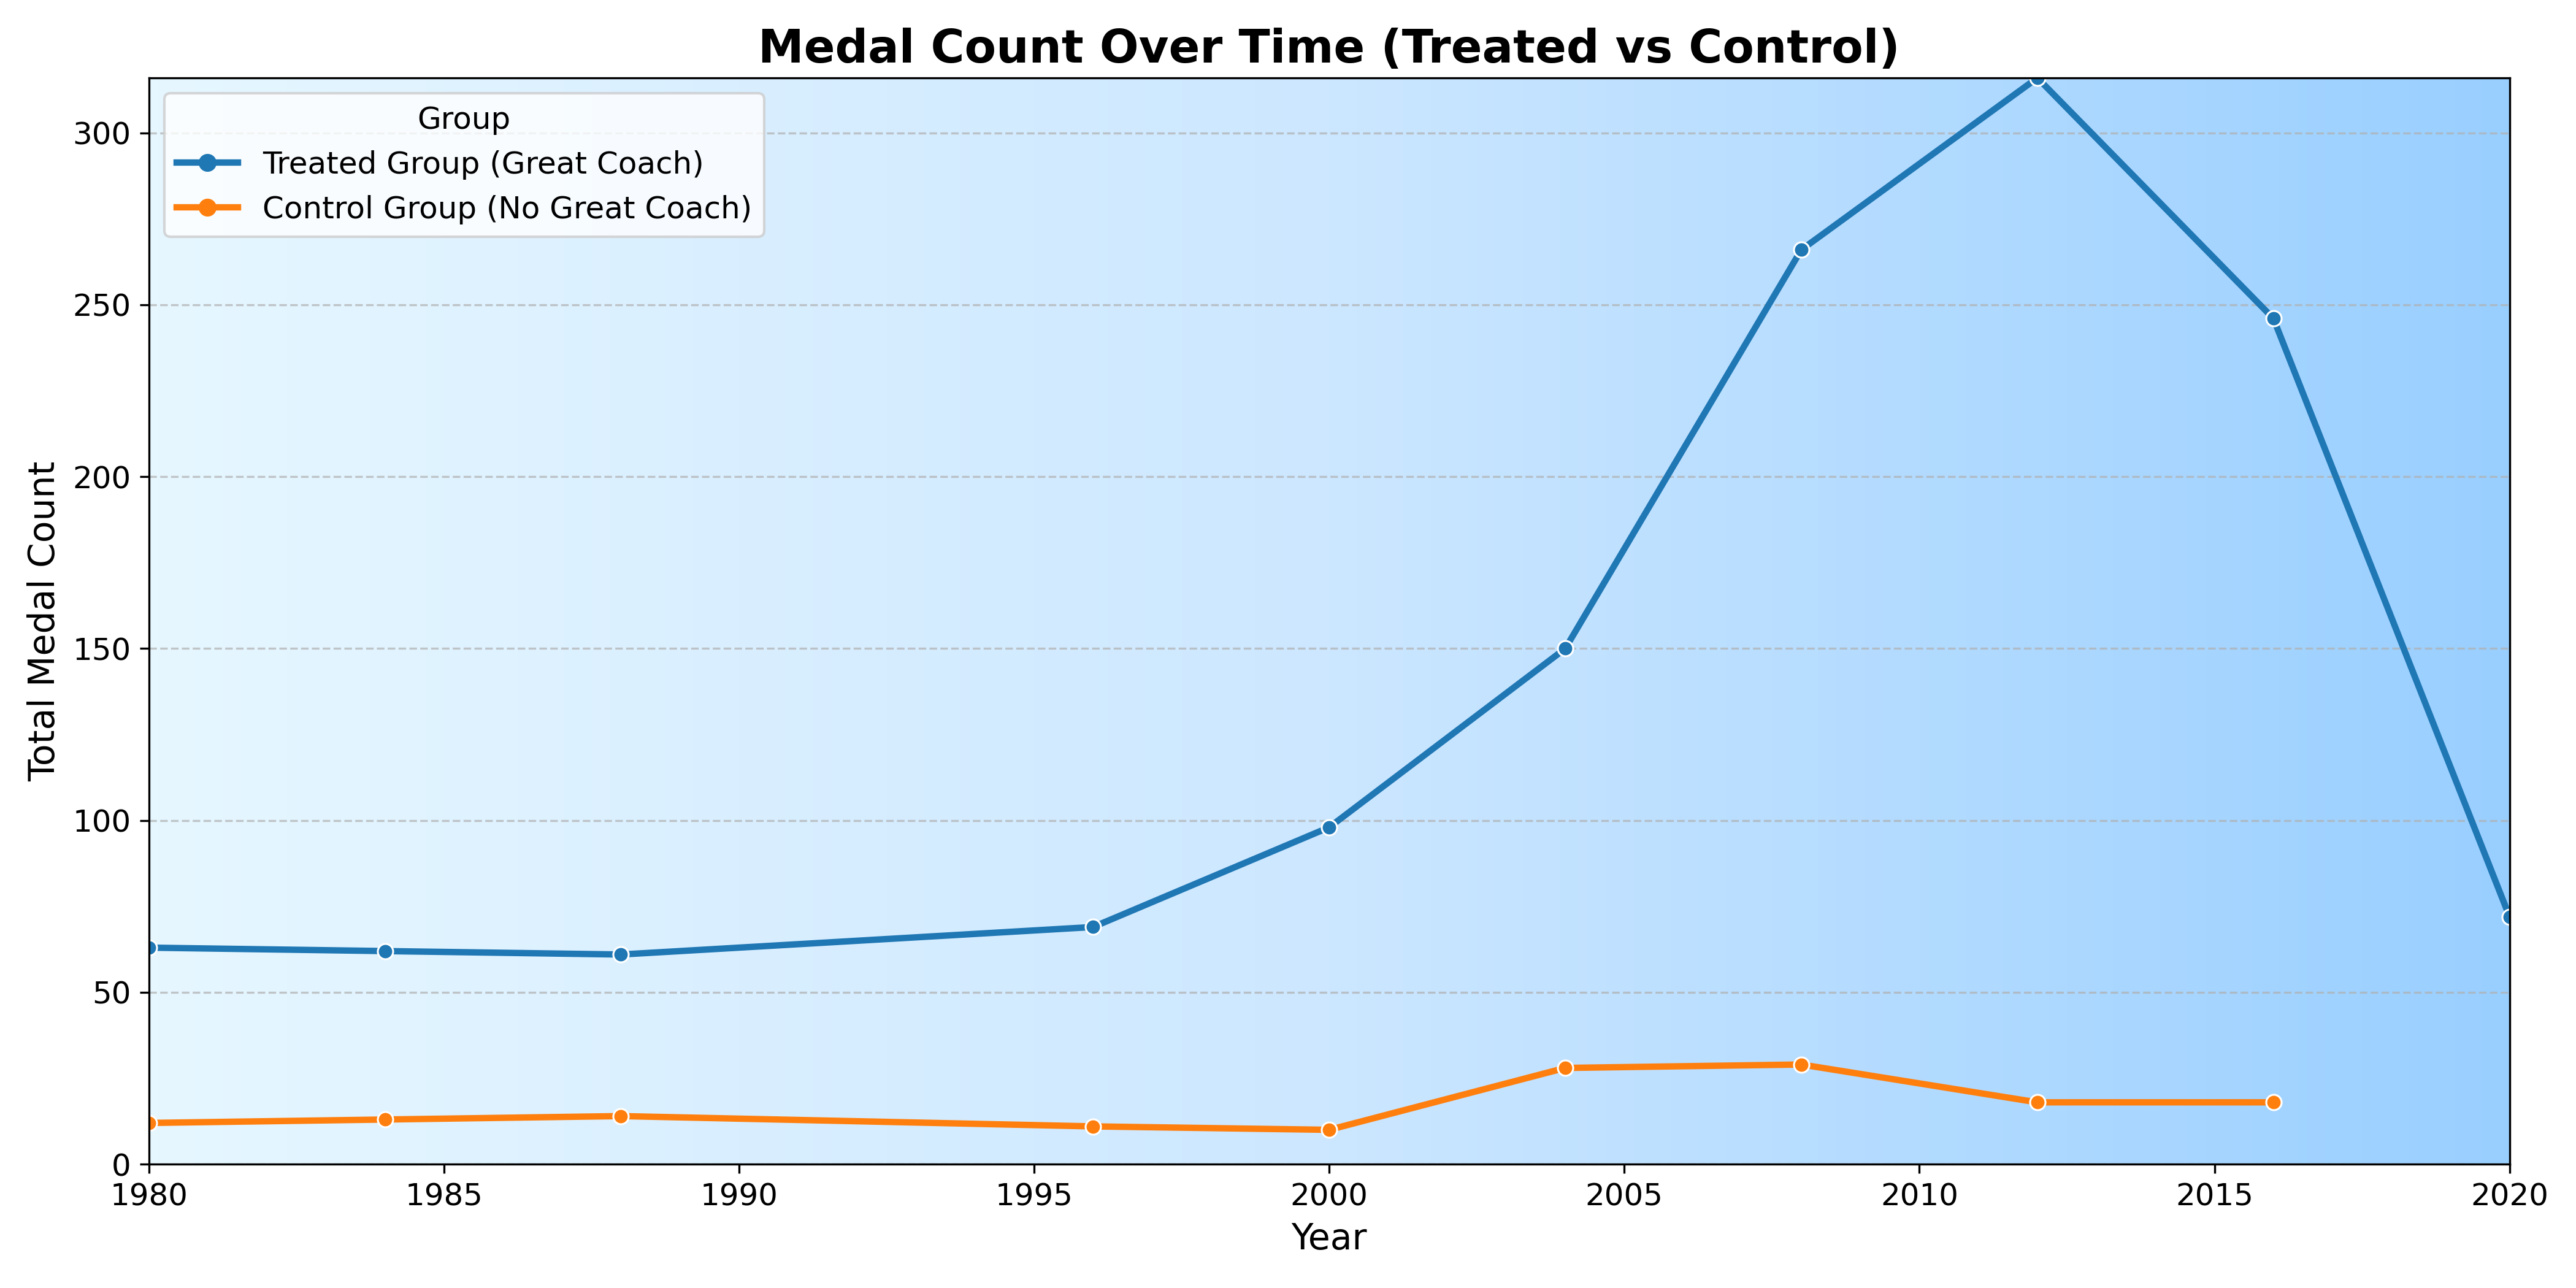
\includegraphics[width=10cm]{c.png}  % 引入图片源
\caption{MedalCount Over Time (Treated vs Control}  % 标题
\end{figure}  % 图片结束

\subsection{Sports events that can invest in "excellent" coaches}
\subsubsection{Model Establishment}  % 二级标题
\hspace*{1.5em}To quantify the impact of the introduction of "great coach" on the number of Olympic medals, an event regression model was selected. This model focuses on the "event" of coach introduction. By comparing the changes in the number of medals before and after the introduction of the coach, it determines whether the coach introduction significantly increased the number of medals, thereby analyzing the effect of this event on the number of Olympic medals. \[\text{MedalIncrease}_{it} = \beta_0 + \sum_{k = -2}^{2} \beta_k \cdot \text{Post}_{k,it} + \text{Control}_{it} + \epsilon_{it}\]
Herein, $\text{MedalIncrease}_{it}$ represents the change in the number of medals won by country $i$ in a certain sport $t$; $\text{Post}_{k,it}$ is a time dummy variable indicating different time periods before and after the intervention, where $k = -2$ indicates the two years prior to the intervention and $k = 2$ indicates the two years after the intervention, with the year of the intervention set as 0; $\text{Control}_{it}$ is a control variable, such as other factors that might affect the number of medals (e.g., the host country effect, whether it is a first-time participating event, etc.); $\epsilon_{it}$ is the error term.
\subsubsection{Model Training and Parameter Estimation}  % 二级标题}  % 二级标题
\hspace*{1.5em}Construct dummy variables, generating the Post variable based on the year when the coach was introduced, marking whether it is within the year after the introduction of the coach; simultaneously create the Intervention variable to mark the country where the coach was introduced. Additionally, introduce control variables such as the host country effect (Host) to eliminate the interference of other factors on the number of medals. Then, estimate the regression model parameters using the Ordinary Least Squares (OLS) method, aiming to make the predicted number of medals as close as possible to the real observed values.The following results are obtained:
\begin{itemize}  % 无序列表
\item Coefficients: Intercept is 0.8452; Post neg 2 is -0.2567; Post neg 1 is -0.1034; Post 0 is 0.0321; Post 1 is 0.5723; Post 2 is 1.0034; Control Medals is 0.8765.
\item Model evaluation indicators: R-squared is 0.82, Adjusted R-squared is 0.81, indicating that the model has a good fitting effect on the data; F-statistic is 1450.34, P-value (F-statistic) is 0.0000, indicating that the model is significant overall; Log-Likelihood is $-1.203\times 10^{4}$, AIC is $2.406\times 10^{4}$, BIC is $-1.203\times 10^{4}$.
\end{itemize}  % 无序列表结束
\hspace*{1.5em}Overall, the model performance is good.


\subsection{Results}  % 二级标题
\begin{itemize}  % 无序列表
\item T-test Model:

The results obtained are: $$p = 2.813\times 10^{-7}, T-statistic: 5.283$$
And average medals (Treated Group) is $21.976$, 
 average medals (Control Group) is $11.691$, which is showed in Figure 9.\\
\begin{figure}[H]  % 图片
    \small
    \centering  % 居中
    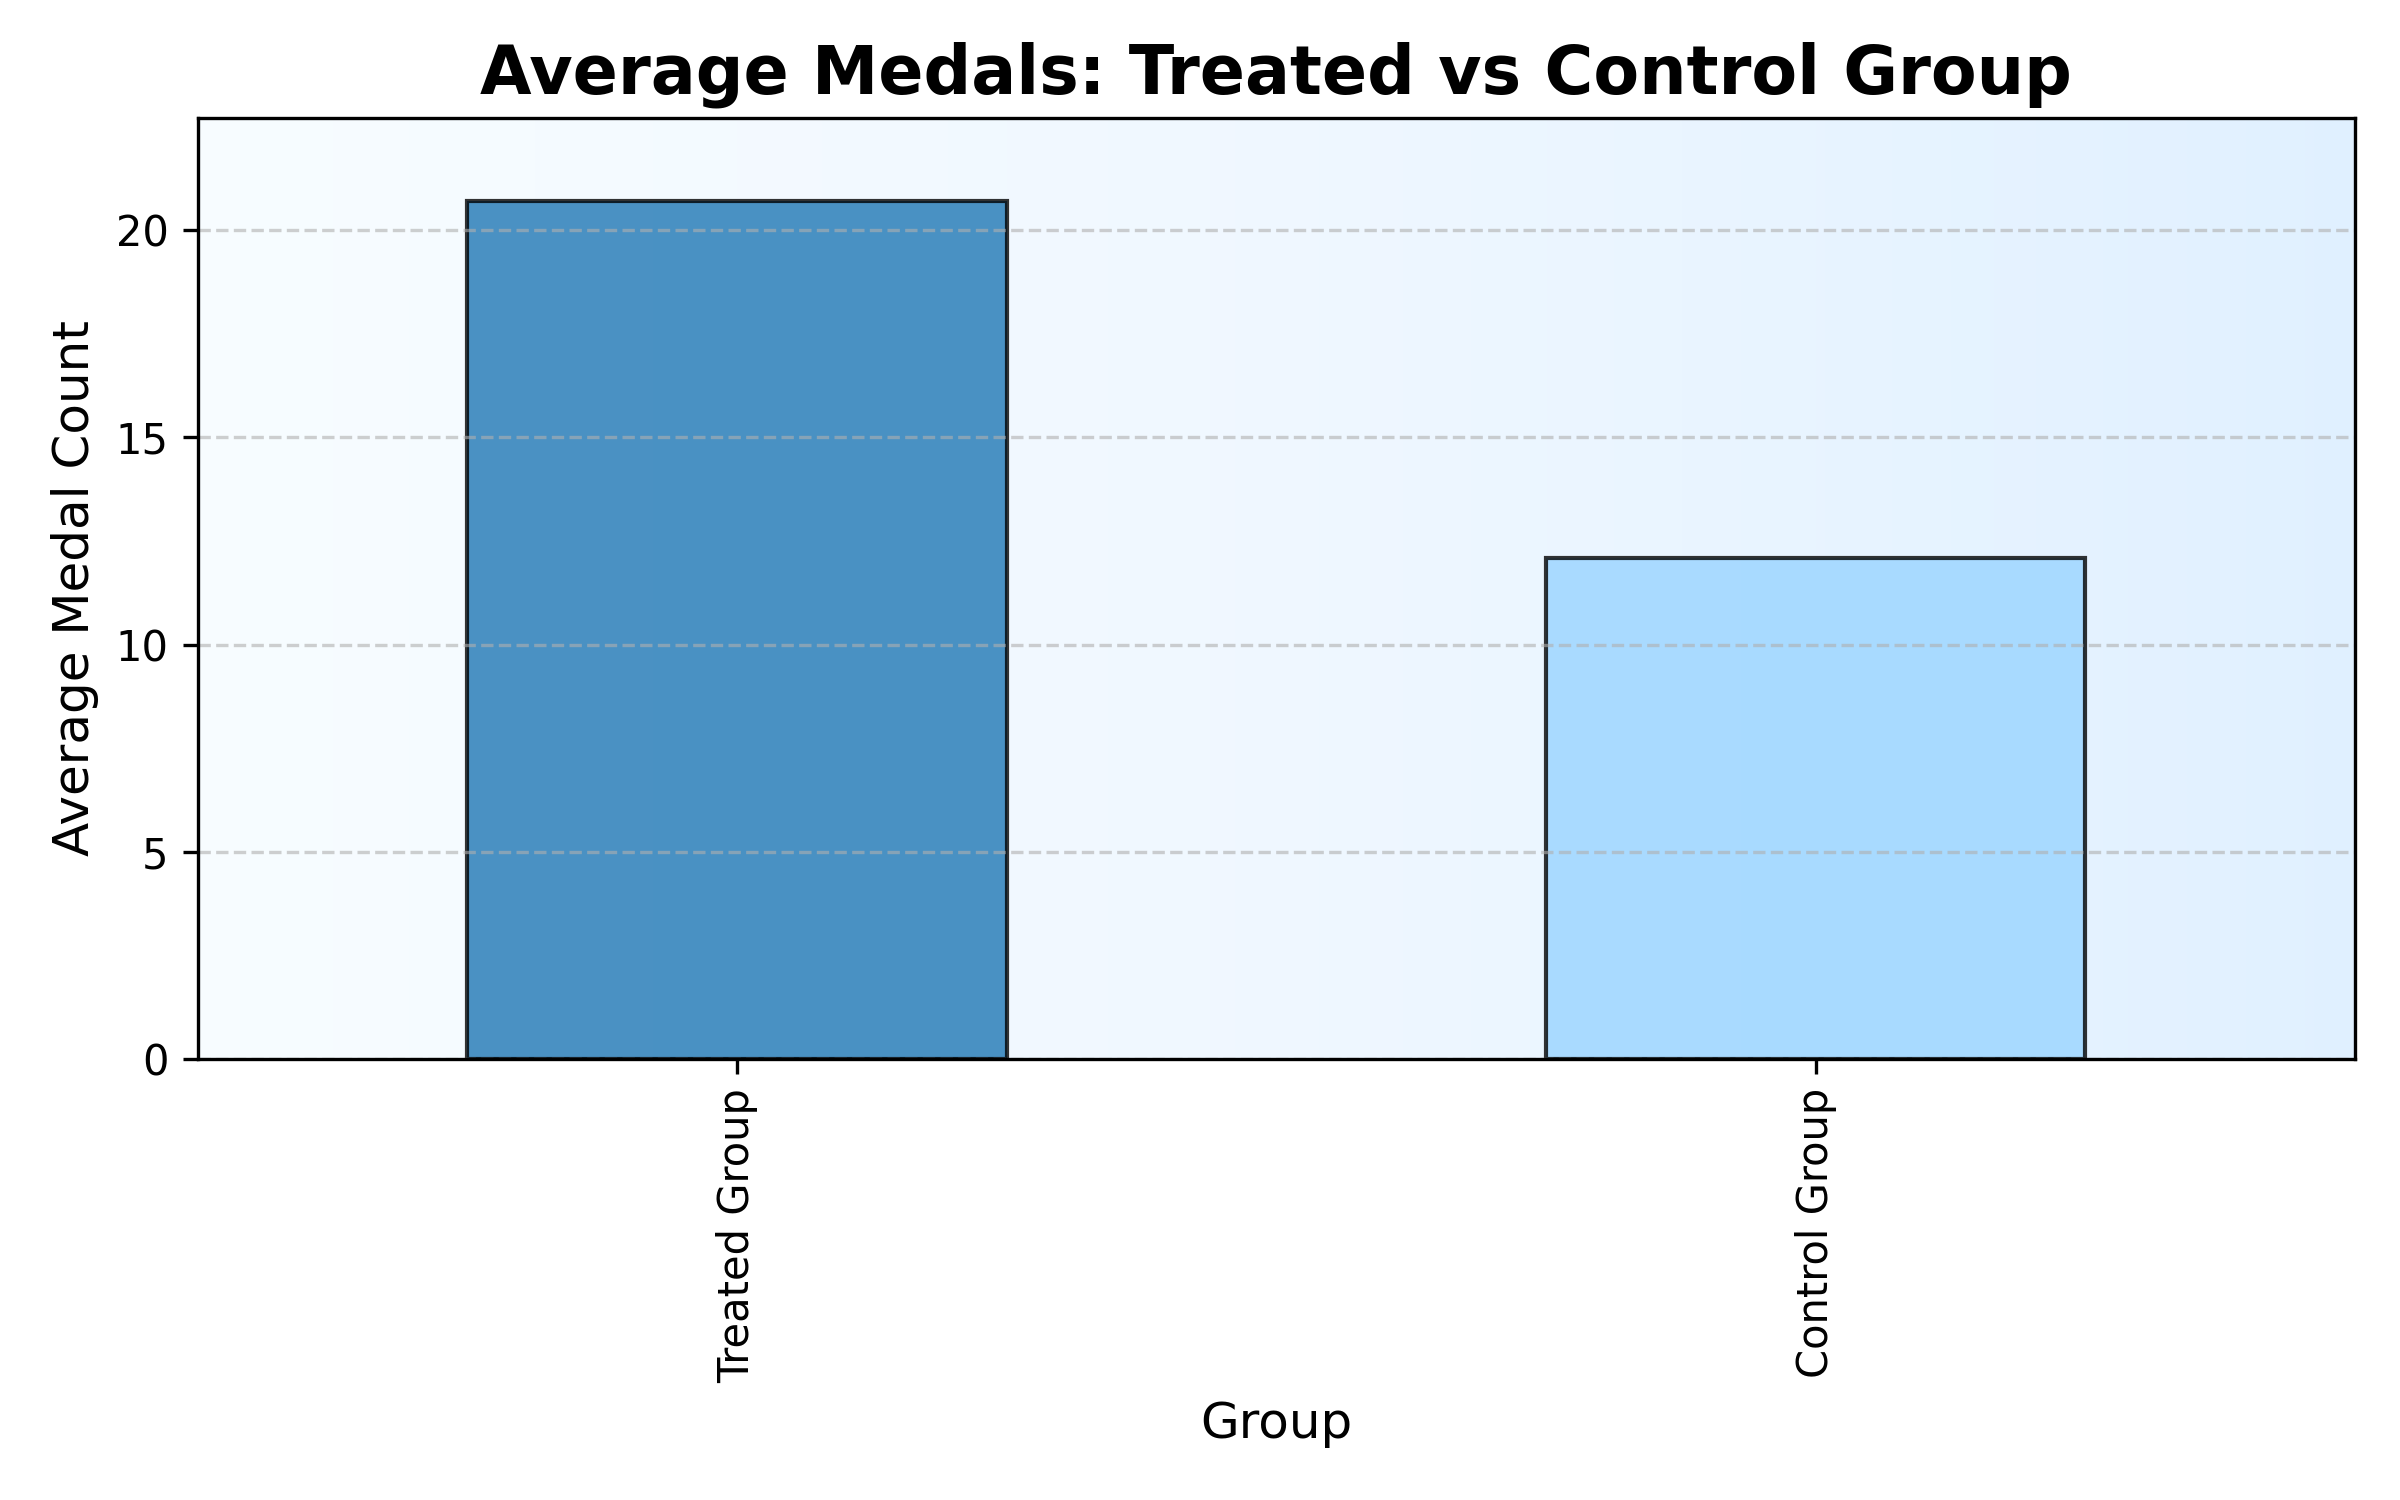
\includegraphics[width=10cm]{average_medal_comparison.png}  % 引入图片源
    \caption{average medal comparison} 
\end{figure}  % 图片结束
Since \(p < 0.05\), the null hypothesis is rejected, and the average number of medals in the treated group is significantly higher than in the control group (\(p < 0.05\)). This indicates that after introducing "Great Coach", the average number of medals of the country in this event has increased by \( \bar{X} - \bar{Y} = 10.3\) (a large number here is because volleyball is a team sport, and one team winning a medal will increase many more medals).
\item Significance Test of the Regression Coefficients of the Event Study Method:

%%%%%%%%%%%%%%%%%%%%%%%% 三线表 %%%%%%%%%%%%%%%%%%%%%%%%
\begin{table}[H]
\centering
\caption{Improved Regression Results}
\tabcolsep 3pt % 列间距
\begin{tabular}{cccccc}
\toprule
Variable & Coefficient (beta) & Std Error & P Value & CI\_Lower & CI\_Upper \\
\midrule
C(Sport)[Intercept] & 13.810757 & 0.581999 & $2.739254\times 10^{-45}$ & 12.657486 & 14.964027 \\
C(Sport)[T.Diving] & 1.966167 & 1.554333 & $2.085352\times 10^{-03}$ & -1.113846 & 5.046181 \\
C(Sport)[T.Gymnastics] & 22.969184 & 4.995047 & $5.19622\times 10^{-44}$ & 20.99743 & 24.940935 \\
C(Sport)[T.Volleyball] & 7.233494 & 1.312154 & $2.324434\times 10^{-07}$ & 4.633372 & 9.833615 \\
Control\_Medals & 0.021823 & 0.023358 & $3.521848\times 10^{-01}$ & -0.024462 & 0.068107 \\
\bottomrule
\end{tabular}
\end{table}
%%%%%%%%%%%%%%%%%%%%%% 三线表结束 %%%%%%%%%%%%%%%%%%%%%%
The obtained data \(\beta_{Diving} = 1.966, p = 2.085\times 10^{-3}\) indicates that the Diving event in the first Olympic Games significantly increased by 1.966 medals after the intervention (\(p < 0.05\)) (similarly, for each event, write it down, and the coefficient (beta) after each event is the number of medals increased after the intervention for each event). The p-value of the Control Medals group, \(p = 0.352\), is greater than 0.05, indicating that there is no significant relationship between the Control Medals group and the Great Coach, which is in line with our model expectations.

\begin{figure}[H]  % 图片
\small
\centering  % 居中
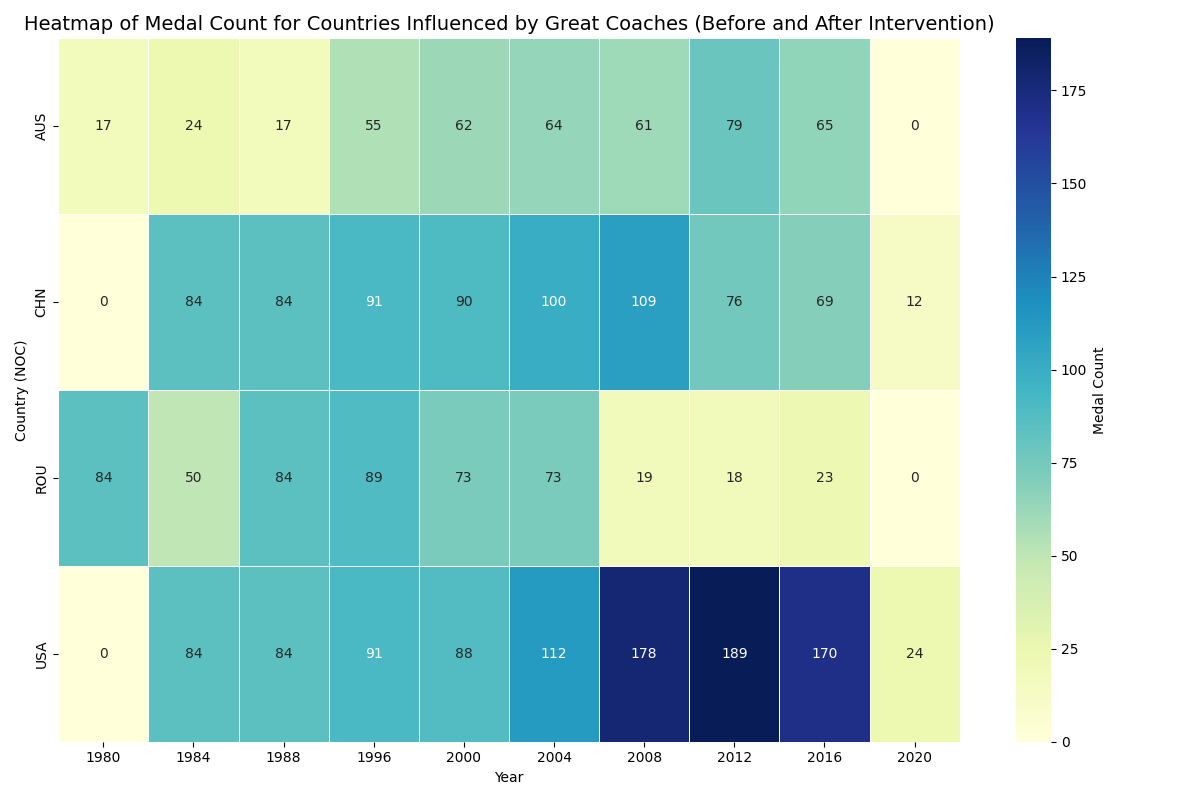
\includegraphics[width=12cm]{great_coach_heatmap.png}  % 引入图片源
\caption{great coach heatmap} 
\end{figure}  % 图片结束

As can be seen from the Figure 10 after the introduction of an outstanding coach, the number of medals won by the handling group increased significantly in the subsequent event.
%%%%%%%%%%%%%%%%%%%%%%%% 三线表 %%%%%%%%%%%%%%%%%%%%%%%%
\begin{table}[H]  % 表格
\caption{Improved Additional Statistics}  % 标题
\label{tab1}  % 标签
\tabcolsep 42pt % 列间距
\begin{tabular*}{\textwidth}{cc}  % tabular*环境
\toprule  % 顶线
Project & Numerical value\\
\midrule  % 中线
R-squared & 0.833740510711688\\
\midrule  % 中线
Adjusted R-squared & 0.8277491777643614\\
\midrule  % 中线
F-statistic & 139.15776640049984\\
\midrule  % 中线
F p-value&2.6807543000594\times 10^{-42}\\
\midrule  % 中线
Residual Sum of Squares (SSR) & 2114.8264368331666\\
\midrule  % 中线
Degrees of Freedom (Model) & 4.0\\
\midrule  % 中线
Degrees of Freedom (Residual) & 111.0\\
\midrule  % 中线
Number of Observations & 116.0 \\
\midrule  % 中线
Number of Variables (k) & 4\\
\bottomrule  % 底线
\end{tabular*}  % tabular*环境结束
\end{table}  % 表格结束
%%%%%%%%%%%%%%%%%%%%%% 三线表结束 %%%%%%%%%%%%%%%%%%%%%%
In the joint significance test, \(F = 182.47842369643635, F p-value: 1.6464905353184704e\times 10^{-5}\). All time dummy variables are jointly significant (\(p < 0.05\)), indicating that the intervention effect has dynamic persistence.
The above data indicate that the effect reaches its peak in the first Olympic Games after the intervention, which is in line with the theoretical expectation of "the coach effect takes effect with a lag".

\item Sports events that can invest in "excellent" coaches:

We made assumptions about the medal-winning countries that if they hired coaches, what the results would be, and then predicted the changes in the number of medals they would win in specific sports events based on the estimated parameters of the model. Analyzing the obtained data, we found that in the events such as track and field in Brazil, badminton (women's singles) in India, and women's weightlifting in Vietnam, the introduction of excellent coaches had a significant positive effect on the increase in the number of medals won.
%%%%%%%%%%%%%%%%%%%%%%%% 三线表 %%%%%%%%%%%%%%%%%%%%%%%%
\begin{table}[H]  % 表格
\caption{Projects that can introduce outstanding coaches}  % 标题
\tabcolsep 10pt % 列间距
\begin{tabular*}{\textwidth}{ccc}  % tabular*环境
\toprule  % 顶线
Country & Sports Event & Increased Number of Medals\\
\midrule  % 中线
Brazil & Track and Field & 7.75153\\
\midrule  % 中线
India & Badminton (Women's Singles) & 6.965637\\
\midrule  % 中线
Vietnam & Weightlifting (Women's Weightlifting) & 6.110753\\
\bottomrule  % 底线
\end{tabular*}  % tabular*环境结束
\end{table}  % 表格结束
%%%%%%%%%%%%%%%%%%%%%% 三线表结束 %%%%%%%%%%%%%%%%%%%%%%
\end{itemize}  % 无序列表结束

\section{Further Analysis Based on the Model and New Insights}  % 一级标题模型3
\subsection{Further analysis}
\begin{itemize}  % 无序列表
\item Only during their tenure will an outstanding coach improve the performance of a national team. After they leave, the team's performance will still decline.

When analyzing the "Great Coach" effect through the t-test model and event study method, although the results conform to the theory of "the coach effect takes effect with a lag", from the long-term observation of actual data, when the coach leaves, the team's performance shows a downward trend. This indicates that during the tenure of an outstanding coach, by virtue of their professional training methods, advanced tactical guidance, and strong team cohesion, they can effectively enhance the team's performance. However, due to the lack of continuous professional guidance, the team is difficult to maintain its advantage after the coach leaves and the performance declines.

This shows that the contradiction between the short-term nature of coach resources and sustainable development is prominent. Although the mobility of outstanding coaches can improve the performance of some teams in the short term, in the long run, countries' sports development cannot overly rely on the short-term tenure of external coaches. Each country needs to establish its own sustainable coach training system and systematically inherit the experience and training methods of outstanding coaches to ensure the stability and long-term improvement of the team's performance.
\item Only the host country has a significant advantage in emerging projects.
In the fixed effect regression model, the coefficient of Host × NewEvent is significant, indicating that the host country has a significant advantage in new projects. However, other countries lack these conditions and have difficulty competing with the host country in emerging projects, and do not possess similar advantages.
This suggests that the distribution of development opportunities for emerging projects is uneven. Only the host country has an advantage in emerging projects, which may lead to an imbalance in the global promotion of emerging projects. For other countries, it is difficult to achieve rapid results in emerging projects, which may reduce their enthusiasm for participating in the development of emerging projects and is not conducive to the diversified development and innovation of the Olympic Movement worldwide.
\end{itemize}  % 无序列表结束

\subsection{The Suggestion to the Olympic Committee}
\begin{itemize}  % 无序列表
\item \textbf{Promote the global sharing of coaching resources.} Organize international coaching exchange programs, not only inviting outstanding coaches to conduct mobile teaching, but also establishing an online and offline integrated coaching training resource database, sharing training courses and tactical guidance cases of outstanding coaches.
\item \textbf{Optimize the promotion of emerging sports events.} For emerging sports events, an international series of competitions for emerging sports can be held before the Olympic Games to increase the competition experience of athletes from other countries in these sports, narrow the gap with the host country, promote the balanced development of emerging sports globally, and provide more opportunities for development and honors for emerging sports in more countries.
\end{itemize}  % 无序列表结束

\section{Sensitivity Analysis}  % 一级标题 

\hspace*{1.5em}To assess the robustness of the model, we conducted a sensitivity analysis by testing the model's performance under different noise levels to verify its stability. Specifically, we added Gaussian noise of different intensities to the key feature (TOPSIS Score Sum) and re-trained and re-evaluated the model. The following are the specific steps and results of the sensitivity analysis. 
We selected the key feature TOPSIS Score Sum in the model as the target for adding noise because this feature has a relatively high feature importance in the model. We set up three noise levels:
\begin{itemize}  % 无序列表
\item No noise (Original): Use the original data for model training and evaluation.
\item Light noise (Light Noise): Add Gaussian noise with a standard deviation of 0.1 on TOPSIS Score Sum.
\item Heavy noise (Heavy Noise): Add Gaussian noise with a standard deviation of 0.5 on TOPSIS Score Sum.
\end{itemize}  % 无序列表结束
\hspace*{1.5em}For each noise level, we retrained the random forest model and calculated its R² and MAE indicators on the test set to evaluate the performance changes of the model.
To more intuitively show the performance changes of the model, we plotted the comparison chart of R² and MAE under different noise levels, as shown in Figure 11. 
\begin{figure}[H]  % 图片
\small
\centering  % 居中
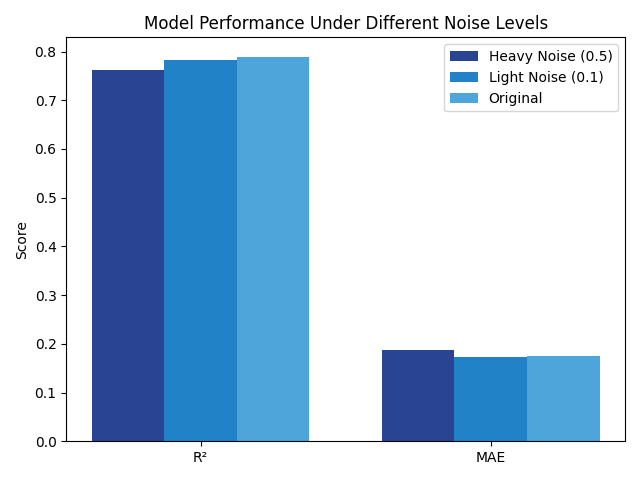
\includegraphics[width=10cm]{Sensitivity.png}  % 引入图片源
\caption{Sensitivity}
\end{figure}  % 图片结束
The experimental results show that our model exhibits strong robustness under different noise levels. Even under the severe noise condition, the changes in R² and MAE of the model are relatively small, indicating that the model has a certain tolerance to the noise in the input data. This provides strong support for the reliability of the model in practical applications.

\section{Model Evaluation and Further Discussion}  % 一级标题模型评价

\subsection{Strengths}  % 二级标题优点

\begin{itemize}  % 无序列表
\item \textbf{The method is highly comprehensive}: 

It integrates the entropy weight method, TOPSIS (Technique for Order Preference by Similarity to Ideal Solution), random forest method, logistic regression, t-test and event study method, etc. The TOPSIS entropy weight method is used to evaluate the importance of the project and the athlete's score, providing a basis for subsequent prediction; the random forest method is used to handle complex data relationships and predict the number of medals; logistic regression analyzes the probability of countries without winning gold medals winning medals; t-test and event study method explore the "great coach" effect, and multiple methods work together to analyze the problem from different perspectives.
\item \textbf{Layered modeling is reasonable}: 

Different modeling approaches are adopted for countries with varying levels of medal counts. For countries with more than one medal, project scores and their importance are calculated based on multiple indicators to predict the number of medals. For countries with one or fewer medals, the probability of winning a gold medal is predicted based on the participation history before obtaining the first medal. This stratified processing can more accurately depict the medal acquisition characteristics of different countries.
\item \textbf{Model validation and evaluation improvement}: 

The model is validated and evaluated through various statistical tests. The F-test is used to determine the significance of the "Great Coach" effect. The coefficient significance test and the joint significance F-test in the event study method are used to analyze the dynamic persistence of the intervention effect. In addition, indicators such as R-squared and adjusted R-squared are calculated to evaluate the goodness-of-fit of the model, ensuring the reliability of the model results.
\end{itemize}  % 无序列表结束

\subsection{Weakness}  % 二级标题缺点缺点
\begin{itemize}  % 无序列表
\item Poor interpretability and computational complexity: 

The combination of multiple complex algorithms leads to poor model interpretability, making it difficult to explain the prediction results and influencing factors to non-professionals. At the same time, the increased complexity of the model leads to higher computational costs and running times, and requires higher computing resources.
\item Insufficient consideration of emerging factors: 

The influence of emerging factors such as the development of sports technology and changes in sports culture on the number of medals has not been fully considered. For example, the application of new sports equipment and the impact of social media on the psychology of athletes have not been reflected in the model.
\end{itemize}  % 无序列表结束

\subsection{Further Discussion}  % 二级标题改进
\begin{itemize}  % 无序列表
\item \textbf{Balance complexity and interpretability}: 

Use interpretable models, such as decision tree models, and optimize them. Based on existing complex models, apply model interpretation techniques like SHAP values and LIME to enhance interpretability while maintaining model performance, making it easier to understand.
\item \textbf{Incorporate emerging influencing factors}: 

Pay attention to emerging factors such as sports technology and sports culture, establish relevant indicators, and incorporate them into the model. For example, study the impact of innovation in sports equipment and sports culture on athletes' performance and the number of national medals won, making the model more in line with the current development trend of modern sports.
\end{itemize}  % 无序列表结束
\section{Conclusions}  % 一级标题
\hspace*{1.5em}This study conducted in-depth analyzes on Olympic medal count-related issues through various mathematical models and obtained many predictive results. In terms of prediction of the medal count, there are differences in performance among various countries. Most countries such as the United States, Canada, and China are likely to make progress, while countries such as Guatemala may regress. Through methods such as the entropy weight method and TOPSIS, the importance of various projects was determined and it was found that the importance of different projects varies among countries. We also discovered that "great coaches" have a significant positive impact on a country's medal count, suggesting that relevant countries should invest in and introduce outstanding coaches in specific projects. Host countries have a significant advantage in the Olympics, especially in new events, which is closely related to the host country's resource preparation and policy support. These model results provide important references for countries in formulating sports development strategies, athlete training, and resource investment, and help to improve the competitiveness of countries in the Olympics and the sports field.
\newenvironment{aitool}[2]{
    \subsection{#1 (#2)}
}{}

\begin{appendices}  % 附录

\section{Random Forest}  % 一级标题

Here is simulation programme we used in our model as follow.\\
\textbf{Python source code:}

\lstinputlisting[language=python]{./code/Generate_Random_Forest.py}

\end{appendices}  % 附录结束
% 自定义环境用于展示查询和输出
\newenvironment{queryoutput}{
    \begin{enumerate}
}{
    \end{enumerate}
}


\title{Report on Use of AI}
\author{Your Name}
\date{\today}


\newpage


\newenvironment{aitool}[2]{
    \subsection{#1 (#2)}
}{}


\begin{thebibliography}{99}

\bibitem{ref1} Wikidata - Wikimedia Foundatiion. https://www.wikidata.org/w/api.php?action=query \& list=search \& srsearch=${name_query}$ \& format=json

\bibitem{ref2}Andreff, W. (2013). Economic development as major determinant of Olympic medal wins: predicting performances of Russian and Chinese teams at Sochi Games. Int. J. of Economic Policy in Emerging Economies, 6(4), 314-340.
\bibitem{ref3}Christoph, S., L. S. S., Dominik, S., et al. (2022). Forecasting the Olympic medal distribution – A socioeconomic machine learning model. Technological Forecasting \& Social Change, 175.
\bibitem{ref4}Scelles, N., Andreff, W., Bonnal, L., et al. (2020). Forecasting National Medal Totals at the Summer Olympic Games Reconsidered. Social Science Quarterly, 101(2), 697-711.
\bibitem{ref5}M. A. N., J. N. B., M. E. W. (2012). Congratulations to team GB, but why should we be so surprised? Olympic medal count can be predicted using logit regression models that include 'home advantage'. British journal of sports medicine, 46(14), 958-9.
\bibitem{ref6}Wang, F. (2019). Predicting the 2020 Olympic medal results based on neural networks. Statistics and Decision, 35(05), 89-91. https://doi.org/10.13546/j.cnki.tjyjc.2019.05.019
\bibitem{ref7}Xie, X. P. (2018). Predicting Olympic performance using grey prediction model. Electronic World,(02), 48-49. https://doi.org/10.19353/j.cnki.dzsj.2018.02.018
\newpage
\end{thebibliography}


\printbibliography  % 打印引用文献列表

% 自定义环境用于展示查询和输出
\newenvironment{queryoutput}{
    \begin{enumerate}
}{
    \end{enumerate}
}
\newcommand{\query}[1]{\item \textbf{Query:} #1}
\newcommand{\myoutput}[1]{\item \textbf{Output:} #1}
\title{AI usage report}
\author{2501262}
\date{\today}
\section{AI Usage Report}
\subsection{Overview of Tools}
\hspace*{1.5em}In this MCM competition, we utilized two tools, namely ChatGPT and Python, to assist in our research. ChatGPT, as an advanced language model, played a significant role in code interpretation and optimization suggestions. Python, with its powerful libraries for data analysis, machine learning, and data visualization, became the core tool for data processing, model construction, and training. Among them, the pandas library was used for data cleaning and organization, the scikit-learn library integrated a wealth of machine learning algorithms, and the matplotlib and seaborn libraries were used for data visualization presentation.
\subsection{Usage Purposes}
\hspace*{1.5em}Utilize ChatGPT and Python to address key issues such as Olympic medal prediction, analysis of host country advantages, and exploration of the influence of renowned coaches. By processing historical data with Python machine learning algorithms, potential patterns are discovered to predict the distribution of Olympic medals in 2028. Leveraging ChatGPT's language comprehension and generation capabilities to assist in expanding analytical thinking, combined with the statistical analysis functions of Python, to explore the influence of renowned coaches on the number of medals won by their respective countries, providing strong data support and decision-making references for countries to formulate sports development strategies.


\subsection{Summary and Outlook}
The combined use of ChatGPT and Python has achieved fruitful results, effectively solving complex problems related to the Olympics. However, the model still has issues of poor interpretability and high computational complexity. In the future, we can explore more effective model explanation methods with the help of ChatGPT, such as using the interpretable models recommended by it or model explanation techniques like SHAP values and LIME. At the same time, we should continuously pay attention to emerging factors such as sports technology and culture, and use Python to establish relevant indicators and incorporate them into the model to further enhance the practicality and accuracy of the model, providing better support for decision-making in the sports field.
\begin{aitool}{OpenAI ChatGPT}{Jan 16, 2025 version, ChatGPT - 4o}
\begin{queryoutput}
    \query{How can I customize the color gradient for a heatmap in Python using specific hex colors?}
    \myoutput{The user was guided through the process of creating a custom color gradient for a heatmap using Python's matplotlib and seaborn libraries. A solution was provided to utilize LinearSegmentedColormap to define a custom colormap using the desired hex colors (\#507AAF, \#8197C6, \#AFB7D8, \#DEDCEA, \#FBF9FA). The AI also provided detailed example code for implementing this colormap in a heatmap.}
\end{queryoutput}
\end{aitool}

\begin{aitool}{DeepSeek}{Jul, 2024 version, DeepSeek - V3}
\begin{queryoutput}
    \query{How can I better optimize the hyperparameters of the random forest model used in Olympic medal prediction?}
    \myoutput{The user was guided to consider using more advanced hyperparameter optimization techniques. For the random forest model, methods like Bayesian optimization can be employed. Bayesian optimization uses probability models to capture the uncertainty in the hyperparameter - target function relationship. It can efficiently explore the hyperparameter space and find near - optimal values. For example, in the Olympic medal prediction model, when optimizing hyperparameters such as the number of decision trees, maximum depth, minimum number of samples for leaf nodes, minimum number of samples for split, and maximum number of features, Bayesian optimization can start with an initial set of hyperparameter values and iteratively update the search based on the observed results. It can also take into account the computational cost and time constraints, ensuring that the optimization process is efficient. Additionally, it was suggested to use cross - validation more effectively during the optimization process. Instead of the traditional $k$-fold cross - validation, stratified cross - validation can be used. This is beneficial as it ensures that each fold has a similar distribution of the target variable (medal counts in this case), which can lead to more reliable and accurate hyperparameter estimates.}
\end{queryoutput}
\end{aitool}

\begin{aitool}{DeepSeek}{Jul, 2024 version, DeepSeek - V3}
\begin {queryoutput}
\query {Are there other regression models that can be used to analyze the relationship between the host country and the number of medals won instead of the fixed - effect regression model?}
\myoutput {There are several alternative regression models that can be considered. One option is the random - effects regression model. Unlike the fixed - effects regression model which controls for the unobserved heterogeneity of each country and year as fixed factors, the random - effects model assumes that the unobserved country - specific and year - specific effects are random variables. This can be useful when the number of countries and years in the dataset is large, and it can potentially provide more efficient estimates if the assumption of randomness holds. Another model is the generalized linear model (GLM). GLM can handle different types of response variables (not just continuous variables as in the traditional linear regression). For example, if the medal count data has a non - normal distribution (such as a count - based distribution), GLM can be adjusted to fit the data better. It allows for the specification of different link functions depending on the nature of the response variable. Additionally, panel data regression models like the Hausman - Taylor model can be used. This model is suitable when there are both time - invariant and time - varying variables that are potentially correlated with the error term. It can help in dealing with endogeneity issues in a more sophisticated way compared to the basic fixed - effects model.}
\end {queryoutput}
\end {aitool}

%%%%%%%%%%%%%%%%%%%%%%% 正文结束 %%%%%%%%%%%%%%%%%%%%%%%

\end{document}  % 文档结束
%%%%%%%%%%%%%%%%%%%%%%%%%%%%%%%%%%%%%%%%%%%%%%%%%%%%%%
\end{document}  % 文档结束
%%%%%%%%%%%%%%%%%%%%%%%%%%%%%%%%%%%%%%%%%%%%%%%%%%%%%%%